\documentclass[]{article}

% Using the caption package allows us to support captions that contain "itemize" environments.
% The font=small option makes the text of captions smaller than the main text.
% Marie asked us to do this.
\usepackage[font=small]{caption}

\usepackage{natbib}
\usepackage{breakcites}
\usepackage{hyperref}
\usepackage{authblk}
\usepackage{amsmath}
\usepackage{graphicx}
\usepackage{bm}

% MIT_TEMPLATE
\newif\ifMIT
%\MITtrue % uncomment to use MIT template
\MITfalse

%%%%% NEW MATH DEFINITIONS %%%%%

% Mark sections of captions for referring to divisions of figures
\newcommand{\figleft}{{\em (Left)}}
\newcommand{\figcenter}{{\em (Center)}}
\newcommand{\figright}{{\em (Right)}}
\newcommand{\figtop}{{\em (Top)}}
\newcommand{\figbottom}{{\em (Bottom)}}
\newcommand{\captiona}{{\em (a)}}
\newcommand{\captionb}{{\em (b)}}
\newcommand{\captionc}{{\em (c)}}
\newcommand{\captiond}{{\em (d)}}

% Highlight a newly defined term
\newcommand{\newterm}[1]{{\bf #1}}


% Figure reference, lower-case.
\def\figref#1{figure~\ref{#1}}
% Figure reference, capital. For start of sentence
\def\Figref#1{Figure~\ref{#1}}
\def\twofigref#1#2{figures \ref{#1} and \ref{#2}}
\def\quadfigref#1#2#3#4{figures \ref{#1}, \ref{#2}, \ref{#3} and \ref{#4}}
% Section reference, lower-case.
\def\secref#1{section~\ref{#1}}
% Section reference, capital.
\def\Secref#1{Section~\ref{#1}}
% Reference to two sections.
\def\twosecrefs#1#2{sections \ref{#1} and \ref{#2}}
% Reference to three sections.
\def\secrefs#1#2#3{sections \ref{#1}, \ref{#2} and \ref{#3}}
% Reference to an equation, lower-case.
\def\eqref#1{equation~\ref{#1}}
% Reference to an equation, upper case
\def\Eqref#1{Equation~\ref{#1}}
% A raw reference to an equation---avoid using if possible
\def\plaineqref#1{\ref{#1}}
% Reference to a chapter, lower-case.
\def\chapref#1{chapter~\ref{#1}}
% Reference to an equation, upper case.
\def\Chapref#1{Chapter~\ref{#1}}
% Reference to a range of chapters
\def\rangechapref#1#2{chapters\ref{#1}--\ref{#2}}
% Reference to an algorithm, lower-case.
\def\algref#1{algorithm~\ref{#1}}
% Reference to an algorithm, upper case.
\def\Algref#1{Algorithm~\ref{#1}}
\def\twoalgref#1#2{algorithms \ref{#1} and \ref{#2}}
\def\Twoalgref#1#2{Algorithms \ref{#1} and \ref{#2}}
% Reference to a part, lower case
\def\partref#1{part~\ref{#1}}
% Reference to a part, upper case
\def\Partref#1{Part~\ref{#1}}
\def\twopartref#1#2{parts \ref{#1} and \ref{#2}}

\def\ceil#1{\lceil #1 \rceil}
\def\floor#1{\lfloor #1 \rfloor}
\def\1{\bm{1}}
\newcommand{\train}{\mathcal{D}}
\newcommand{\valid}{\mathcal{D_{\mathrm{valid}}}}
\newcommand{\test}{\mathcal{D_{\mathrm{test}}}}

\def\eps{{\epsilon}}


% Random variables
\def\reta{{\textnormal{$\eta$}}}
\def\ra{{\textnormal{a}}}
\def\rb{{\textnormal{b}}}
\def\rc{{\textnormal{c}}}
\def\rd{{\textnormal{d}}}
\def\re{{\textnormal{e}}}
\def\rf{{\textnormal{f}}}
\def\rg{{\textnormal{g}}}
\def\rh{{\textnormal{h}}}
\def\ri{{\textnormal{i}}}
\def\rj{{\textnormal{j}}}
\def\rk{{\textnormal{k}}}
\def\rl{{\textnormal{l}}}
%\def\rm{{\textnormal{m}}}
\def\rn{{\textnormal{n}}}
\def\ro{{\textnormal{o}}}
\def\rp{{\textnormal{p}}}
\def\rq{{\textnormal{q}}}
\def\rr{{\textnormal{r}}}
\def\rs{{\textnormal{s}}}
\def\rt{{\textnormal{t}}}
\def\ru{{\textnormal{u}}}
\def\rv{{\textnormal{v}}}
\def\rw{{\textnormal{w}}}
\def\rx{{\textnormal{x}}}
\def\ry{{\textnormal{y}}}
\def\rz{{\textnormal{z}}}

% Random vectors
\def\rvepsilon{{\mathbf{\epsilon}}}
\def\rvtheta{{\mathbf{\theta}}}
\def\rva{{\mathbf{a}}}
\def\rvb{{\mathbf{b}}}
\def\rvc{{\mathbf{c}}}
\def\rvd{{\mathbf{d}}}
\def\rve{{\mathbf{e}}}
\def\rvf{{\mathbf{f}}}
\def\rvg{{\mathbf{g}}}
\def\rvh{{\mathbf{h}}}
\def\rvu{{\mathbf{i}}}
\def\rvj{{\mathbf{j}}}
\def\rvk{{\mathbf{k}}}
\def\rvl{{\mathbf{l}}}
\def\rvm{{\mathbf{m}}}
\def\rvn{{\mathbf{n}}}
\def\rvo{{\mathbf{o}}}
\def\rvp{{\mathbf{p}}}
\def\rvq{{\mathbf{q}}}
\def\rvr{{\mathbf{r}}}
\def\rvs{{\mathbf{s}}}
\def\rvt{{\mathbf{t}}}
\def\rvu{{\mathbf{u}}}
\def\rvv{{\mathbf{v}}}
\def\rvw{{\mathbf{w}}}
\def\rvx{{\mathbf{x}}}
\def\rvy{{\mathbf{y}}}
\def\rvz{{\mathbf{z}}}

% Elements of random vectors
\def\erva{{\textnormal{a}}}
\def\ervb{{\textnormal{b}}}
\def\ervc{{\textnormal{c}}}
\def\ervd{{\textnormal{d}}}
\def\erve{{\textnormal{e}}}
\def\ervf{{\textnormal{f}}}
\def\ervg{{\textnormal{g}}}
\def\ervh{{\textnormal{h}}}
\def\ervi{{\textnormal{i}}}
\def\ervj{{\textnormal{j}}}
\def\ervk{{\textnormal{k}}}
\def\ervl{{\textnormal{l}}}
\def\ervm{{\textnormal{m}}}
\def\ervn{{\textnormal{n}}}
\def\ervo{{\textnormal{o}}}
\def\ervp{{\textnormal{p}}}
\def\ervq{{\textnormal{q}}}
\def\ervr{{\textnormal{r}}}
\def\ervs{{\textnormal{s}}}
\def\ervt{{\textnormal{t}}}
\def\ervu{{\textnormal{u}}}
\def\ervv{{\textnormal{v}}}
\def\ervw{{\textnormal{w}}}
\def\ervx{{\textnormal{x}}}
\def\ervy{{\textnormal{y}}}
\def\ervz{{\textnormal{z}}}

% Random matrices
\def\rmA{{\mathbf{A}}}
\def\rmB{{\mathbf{B}}}
\def\rmC{{\mathbf{C}}}
\def\rmD{{\mathbf{D}}}
\def\rmE{{\mathbf{E}}}
\def\rmF{{\mathbf{F}}}
\def\rmG{{\mathbf{G}}}
\def\rmH{{\mathbf{H}}}
\def\rmI{{\mathbf{I}}}
\def\rmJ{{\mathbf{J}}}
\def\rmK{{\mathbf{K}}}
\def\rmL{{\mathbf{L}}}
\def\rmM{{\mathbf{M}}}
\def\rmN{{\mathbf{N}}}
\def\rmO{{\mathbf{O}}}
\def\rmP{{\mathbf{P}}}
\def\rmQ{{\mathbf{Q}}}
\def\rmR{{\mathbf{R}}}
\def\rmS{{\mathbf{S}}}
\def\rmT{{\mathbf{T}}}
\def\rmU{{\mathbf{U}}}
\def\rmV{{\mathbf{V}}}
\def\rmW{{\mathbf{W}}}
\def\rmX{{\mathbf{X}}}
\def\rmY{{\mathbf{Y}}}
\def\rmZ{{\mathbf{Z}}}

% Elements of random matrices
\def\ermA{{\textnormal{A}}}
\def\ermB{{\textnormal{B}}}
\def\ermC{{\textnormal{C}}}
\def\ermD{{\textnormal{D}}}
\def\ermE{{\textnormal{E}}}
\def\ermF{{\textnormal{F}}}
\def\ermG{{\textnormal{G}}}
\def\ermH{{\textnormal{H}}}
\def\ermI{{\textnormal{I}}}
\def\ermJ{{\textnormal{J}}}
\def\ermK{{\textnormal{K}}}
\def\ermL{{\textnormal{L}}}
\def\ermM{{\textnormal{M}}}
\def\ermN{{\textnormal{N}}}
\def\ermO{{\textnormal{O}}}
\def\ermP{{\textnormal{P}}}
\def\ermQ{{\textnormal{Q}}}
\def\ermR{{\textnormal{R}}}
\def\ermS{{\textnormal{S}}}
\def\ermT{{\textnormal{T}}}
\def\ermU{{\textnormal{U}}}
\def\ermV{{\textnormal{V}}}
\def\ermW{{\textnormal{W}}}
\def\ermX{{\textnormal{X}}}
\def\ermY{{\textnormal{Y}}}
\def\ermZ{{\textnormal{Z}}}

% Vectors
\def\vzero{{\bm{0}}}
\def\vone{{\bm{1}}}
\def\va{{\bm{a}}}
\def\vb{{\bm{b}}}
\def\vc{{\bm{c}}}
\def\vd{{\bm{d}}}
\def\ve{{\bm{e}}}
\def\vf{{\bm{f}}}
\def\vg{{\bm{g}}}
\def\vh{{\bm{h}}}
\def\vi{{\bm{i}}}
\def\vj{{\bm{j}}}
\def\vk{{\bm{k}}}
\def\vl{{\bm{l}}}
\def\vm{{\bm{m}}}
\def\vn{{\bm{n}}}
\def\vo{{\bm{o}}}
\def\vp{{\bm{p}}}
\def\vq{{\bm{q}}}
\def\vr{{\bm{r}}}
\def\vs{{\bm{s}}}
\def\vt{{\bm{t}}}
\def\vu{{\bm{u}}}
\def\vv{{\bm{v}}}
\def\vw{{\bm{w}}}
\def\vx{{\bm{x}}}
\def\vy{{\bm{y}}}
\def\vz{{\bm{z}}}
\ifMIT
% MIT_TEMPLATE : \bm{\lambda} was generating missing fonts,
% probably because \newcommand{\bmmax}{1} removed them.
% I think \boldmath should be very similar.
\def\vlambda{{\boldmath{\lambda}}}
\def\vmu{{\boldmath{\mu}}}
\def\valpha{{\boldmath{\alpha}}}
\def\vbeta{{\boldmath{\beta}}}
\def\gamma{{\boldmath{\vgamma}}}
\def\vtheta{{\boldmath{\theta}}}
\def\vepsilon{{\boldmath{\epsilon}}}
\def\vomega{{\boldmath{\omega}}}
\def\vpsi{{\boldmath{\psi}}}
\def\vsigma{{\boldmath{\sigma}}}
\def\vSigma{{\boldmath{\Sigma}}}
\def\veta{{\boldmath{\eta}}}
\def\vrho{{\boldmath{\rho}}}
\def\vRho{{\boldmath{\Rho}}}
\def\vphi{{\boldmath{\phi}}}
\def\vPhi{{\boldmath{\Phi}}}
\def\vDelta{{\boldmath{\Delta}}}
\def\vdelta{{\boldmath{\delta}}}
\else
\def\vlambda{{\bm{\lambda}}}
\def\vmu{{\bm{\mu}}}
\def\valpha{{\bm{\alpha}}}
\def\vbeta{{\bm{\beta}}}
\def\vgamma{{\bm{\gamma}}}
\def\vtheta{{\bm{\theta}}}
\def\vepsilon{{\bm{\epsilon}}}
\def\vomega{{\bm{\omega}}}
\def\vpsi{{\bm{\psi}}}
\def\vphi{{\bm{\phi}}}
\def\vsigma{{\bm{\sigma}}}
\def\vSigma{{\bm{\Sigma}}}
\def\veta{{\bm{\eta}}}
\def\vrho{{\bm{\rho}}}
\def\vRho{{\bm{\Rho}}}
\def\vphi{{\bm{\phi}}}
\def\vPhi{{\bm{\Phi}}}
\def\vDelta{{\bm{\Delta}}}
\def\vdelta{{\bm{\delta}}}
\fi

%\def\KeyIdea{{\marginpar{KEY IDEA}}}
% YB: until we populate the book more thoroughly with KEY IDEA, probably best to leave this out
\def\KeyIdea{}

% Elements of vectors
\def\evalpha{{\alpha}}
\def\evbeta{{\beta}}
\def\evepsilon{{\epsilon}}
\def\evlambda{{\lambda}}
\def\evomega{{\omega}}
\def\evmu{{\mu}}
\def\evpsi{{\psi}}
\def\evsigma{{\sigma}}
\def\evtheta{{\theta}}
\def\eva{{a}}
\def\evb{{b}}
\def\evc{{c}}
\def\evd{{d}}
\def\eve{{e}}
\def\evf{{f}}
\def\evg{{g}}
\def\evh{{h}}
\def\evi{{i}}
\def\evj{{j}}
\def\evk{{k}}
\def\evl{{l}}
\def\evm{{m}}
\def\evn{{n}}
\def\evo{{o}}
\def\evp{{p}}
\def\evq{{q}}
\def\evr{{r}}
\def\evs{{s}}
\def\evt{{t}}
\def\evu{{u}}
\def\evv{{v}}
\def\evw{{w}}
\def\evx{{x}}
\def\evy{{y}}
\def\evz{{z}}

% Matrix
\def\mA{{\bm{A}}}
\def\mB{{\bm{B}}}
\def\mC{{\bm{C}}}
\def\mD{{\bm{D}}}
\def\mE{{\bm{E}}}
\def\mF{{\bm{F}}}
\def\mG{{\bm{G}}}
\def\mH{{\bm{H}}}
\def\mI{{\bm{I}}}
\def\mJ{{\bm{J}}}
\def\mK{{\bm{K}}}
\def\mL{{\bm{L}}}
\def\mM{{\bm{M}}}
\def\mN{{\bm{N}}}
\def\mO{{\bm{O}}}
\def\mP{{\bm{P}}}
\def\mQ{{\bm{Q}}}
\def\mR{{\bm{R}}}
\def\mS{{\bm{S}}}
\def\mT{{\bm{T}}}
\def\mU{{\bm{U}}}
\def\mV{{\bm{V}}}
\def\mW{{\bm{W}}}
\def\mX{{\bm{X}}}
\def\mY{{\bm{Y}}}
\def\mZ{{\bm{Z}}}
\ifMIT
\def\mLambda{{\boldmath{\Lambda}}}
\def\mBeta{{\boldmath{\beta}}}
\def\mPhi{{\boldmath{\Phi}}}
\def\mSigma{{\boldmath{\Sigma}}}
\else
\def\mBeta{{\bm{\beta}}}
\def\mPhi{{\bm{\Phi}}}
\def\mLambda{{\bm{\Lambda}}}
\def\mSigma{{\bm{\Sigma}}}
\fi

% Tensor
% Got this from here: http://tex.stackexchange.com/questions/77640/bold-italic-and-sans-serif-math-symbols
\DeclareMathAlphabet{\mathsfit}{\encodingdefault}{\sfdefault}{m}{sl}
\SetMathAlphabet{\mathsfit}{bold}{\encodingdefault}{\sfdefault}{bx}{n}
\newcommand{\tens}[1]{\bm{\mathsfit{#1}}}
\def\tA{{\tens{A}}}
\def\tB{{\tens{B}}}
\def\tC{{\tens{C}}}
\def\tD{{\tens{D}}}
\def\tE{{\tens{E}}}
\def\tF{{\tens{F}}}
\def\tG{{\tens{G}}}
\def\tH{{\tens{H}}}
\def\tI{{\tens{I}}}
\def\tJ{{\tens{J}}}
\def\tK{{\tens{K}}}
\def\tL{{\tens{L}}}
\def\tM{{\tens{M}}}
\def\tN{{\tens{N}}}
\def\tO{{\tens{O}}}
\def\tP{{\tens{P}}}
\def\tQ{{\tens{Q}}}
\def\tR{{\tens{R}}}
\def\tS{{\tens{S}}}
\def\tT{{\tens{T}}}
\def\tU{{\tens{U}}}
\def\tV{{\tens{V}}}
\def\tW{{\tens{W}}}
\def\tX{{\tens{X}}}
\def\tY{{\tens{Y}}}
\def\tZ{{\tens{Z}}}


% Graph
\def\gA{{\mathcal{A}}}
\def\gB{{\mathcal{B}}}
\def\gC{{\mathcal{C}}}
\def\gD{{\mathcal{D}}}
\def\gE{{\mathcal{E}}}
\def\gF{{\mathcal{F}}}
\def\gG{{\mathcal{G}}}
\def\gH{{\mathcal{H}}}
\def\gI{{\mathcal{I}}}
\def\gJ{{\mathcal{J}}}
\def\gK{{\mathcal{K}}}
\def\gL{{\mathcal{L}}}
\def\gM{{\mathcal{M}}}
\def\gN{{\mathcal{N}}}
\def\gO{{\mathcal{O}}}
\def\gP{{\mathcal{P}}}
\def\gQ{{\mathcal{Q}}}
\def\gR{{\mathcal{R}}}
\def\gS{{\mathcal{S}}}
\def\gT{{\mathcal{T}}}
\def\gU{{\mathcal{U}}}
\def\gV{{\mathcal{V}}}
\def\gW{{\mathcal{W}}}
\def\gX{{\mathcal{X}}}
\def\gY{{\mathcal{Y}}}
\def\gZ{{\mathcal{Z}}}

% Sets
\def\sA{{\mathbb{A}}}
\def\sB{{\mathbb{B}}}
\def\sC{{\mathbb{C}}}
\def\sD{{\mathbb{D}}}
% Don't use a set called E, because this would be the same as our symbol
% for expectation.
\def\sF{{\mathbb{F}}}
\def\sG{{\mathbb{G}}}
\def\sH{{\mathbb{H}}}
\def\sI{{\mathbb{I}}}
\def\sJ{{\mathbb{J}}}
\def\sK{{\mathbb{K}}}
\def\sL{{\mathbb{L}}}
\def\sM{{\mathbb{M}}}
\def\sN{{\mathbb{N}}}
\def\sO{{\mathbb{O}}}
\def\sP{{\mathbb{P}}}
\def\sQ{{\mathbb{Q}}}
\def\sR{{\mathbb{R}}}
\def\sS{{\mathbb{S}}}
\def\sT{{\mathbb{T}}}
\def\sU{{\mathbb{U}}}
\def\sV{{\mathbb{V}}}
\def\sW{{\mathbb{W}}}
\def\sX{{\mathbb{X}}}
\def\sY{{\mathbb{Y}}}
\def\sZ{{\mathbb{Z}}}

% Matrix elements
% NOTE: we changed these from lower case to upper case to avoid
% clashes between vectors and matrices with same letter name.
% For example, we don't want elements of the hidden layer vector
% h to have the same name as elements of the Hessian matrix H
\def\emLambda{{\Lambda}}
\def\emA{{A}}
\def\emB{{B}}
\def\emC{{C}}
\def\emD{{D}}
\def\emE{{E}}
\def\emF{{F}}
\def\emG{{G}}
\def\emH{{H}}
\def\emI{{I}}
\def\emJ{{J}}
\def\emK{{K}}
\def\emL{{L}}
\def\emM{{M}}
\def\emN{{N}}
\def\emO{{O}}
\def\emP{{P}}
\def\emQ{{Q}}
\def\emR{{R}}
\def\emS{{S}}
\def\emT{{T}}
\def\emU{{U}}
\def\emV{{V}}
\def\emW{{W}}
\def\emX{{X}}
\def\emY{{Y}}
\def\emZ{{Z}}
\def\emSigma{{\Sigma}}

% Tensor elements
% Same font as tensor, without \bm wrapper
\newcommand{\etens}[1]{\mathsfit{#1}}
\def\etLambda{{\etens{\Lambda}}}
\def\etA{{\etens{A}}}
\def\etB{{\etens{B}}}
\def\etC{{\etens{C}}}
\def\etD{{\etens{D}}}
\def\etE{{\etens{E}}}
\def\etF{{\etens{F}}}
\def\etG{{\etens{G}}}
\def\etH{{\etens{H}}}
\def\etI{{\etens{I}}}
\def\etJ{{\etens{J}}}
\def\etK{{\etens{K}}}
\def\etL{{\etens{L}}}
\def\etM{{\etens{M}}}
\def\etN{{\etens{N}}}
\def\etO{{\etens{O}}}
\def\etP{{\etens{P}}}
\def\etQ{{\etens{Q}}}
\def\etR{{\etens{R}}}
\def\etS{{\etens{S}}}
\def\etT{{\etens{T}}}
\def\etU{{\etens{U}}}
\def\etV{{\etens{V}}}
\def\etW{{\etens{W}}}
\def\etX{{\etens{X}}}
\def\etY{{\etens{Y}}}
\def\etZ{{\etens{Z}}}

% The true underlying data generating distribution
\newcommand{\pdata}{p_{\rm{data}}}
% The empirical distribution defined by the training set
\newcommand{\ptrain}{\hat{p}_{\rm{data}}}
\def\empirical{\ptrain} % Accidental duplicate
\newcommand{\Ptrain}{\hat{P}_{\rm{data}}}
% The model distribution
\newcommand{\pmodel}{p_{\rm{model}}}
\newcommand{\Pmodel}{P_{\rm{model}}}
\newcommand{\ptildemodel}{\tilde{p}_{\rm{model}}}
% Stochastic autoencoder distributions
\newcommand{\pencode}{p_{\rm{encoder}}}
\newcommand{\pdecode}{p_{\rm{decoder}}}
\newcommand{\precons}{p_{\rm{reconstruct}}}

\newcommand{\laplace}{\mathrm{Laplace}} % Laplace distribution, see first use in prob.tex

\newcommand{\E}{\mathbb{E}}
\newcommand{\Ls}{\mathcal{L}}
\newcommand{\R}{\mathbb{R}}
\newcommand{\emp}{\tilde{p}}
\newcommand{\lr}{\alpha}
\newcommand{\reg}{\lambda}
\newcommand{\rect}{\mathrm{rectifier}}
\newcommand{\softmax}{\mathrm{softmax}}
\newcommand{\sigmoid}{\sigma} % Note: main text often hardcodes \sigma still, also
% many equations would likely frame bust if expanded to say \mathrm{sigmoid}
\newcommand{\sigm}{\sigmoid} % Duplicate command, this one is deprecated
\newcommand{\softplus}{\zeta} % Note: some figures may not use this macro, but main text consistently does
\newcommand{\KL}{D_{\mathrm{KL}}}
\newcommand{\Var}{\mathrm{Var}}
\newcommand{\standarderror}{\mathrm{SE}}
\newcommand{\Cov}{\mathrm{Cov}}
% Put these here so we can keep same syntax throughout the book but also change
% it easily.
% Wolfram Mathworld says $L^2$ is for function spaces and $\ell^2$ is for vectors
% But then they seem to use $L^2$ for vectors throughout the site, and so does
% wikipedia.
% No one really seems to use subscripts (l_2, L_2) on general math reference
% sites, though subscripts seem popular in machine learning.
\newcommand{\normlzero}{L^0}
\newcommand{\normlone}{L^1}
\newcommand{\normltwo}{L^2}
\newcommand{\normlp}{L^p}
\newcommand{\normmax}{L^\infty}

% NOTE: This one was not done with a macro originally, many uses need to converted
% to \parents rather than Pa if we want to change it.
\newcommand{\parents}{Pa} % See usage in notation.tex. Chosen to match Daphne's book.

\ifMIT
\else
\DeclareMathOperator*{\argmax}{arg\,max}
\DeclareMathOperator*{\argmin}{arg\,min}
\fi
\DeclareMathOperator{\sign}{sign}
\DeclareMathOperator{\Tr}{Tr}
\let\ab\allowbreak


\title{NIPS 2016 Tutorial:\\ Generative Adversarial Networks}

\author{Ian Goodfellow}
\affil{OpenAI, {\tt ian@openai.com}}

\renewcommand\Authands{, and }


\date{}

\begin{document}

\maketitle

\begin{abstract}
This report summarizes the tutorial presented by the author at NIPS 2016 on
{\em generative adversarial networks} (GANs).
The tutorial describes:
(1) Why generative modeling is a topic worth studying,
(2) how generative models work, and how GANs compare to other generative models,
(3) the details of how GANs work,
(4) research frontiers in GANs, and
(5) state-of-the-art image models that combine GANs with other methods.
Finally, the tutorial contains three exercises for readers to complete,
and the solutions to these exercises.
\end{abstract}


\section*{Introduction}


This report\footnote{This is the arxiv.org version of this tutorial.
  Some graphics have been compressed to respect arxiv.org's 10MB limit on paper size,
  and do not reflect the full image quality.
}
summarizes the content of the NIPS 2016 tutorial on {\em generative adversarial networks}
(GANs) \citep{Goodfellow-et-al-NIPS2014-small}.
The tutorial was designed primarily to ensure that it answered most of
the questions asked by audience members ahead of time, in order to make sure
that the tutorial would be as useful as possible to the audience.
This tutorial is not intended to be a comprehensive review of the field
of GANs; many excellent papers are not described here, simply because
they were not relevant to answering the most frequent questions, and because
the tutorial was delivered as a two hour oral presentation and did not
have unlimited time cover all subjects.

The tutorial describes:
(1) Why generative modeling is a topic worth studying,
(2) how generative models work, and how GANs compare to other generative models,
(3) the details of how GANs work,
(4) research frontiers in GANs, and
(5) state-of-the-art image models that combine GANs with other methods.
Finally, the tutorial contains three exercises for readers to complete,
and the solutions to these exercises.

The slides for the tutorial are available in PDF and Keynote format at the following URLs:

\url{http://www.iangoodfellow.com/slides/2016-12-04-NIPS.pdf}

\url{http://www.iangoodfellow.com/slides/2016-12-04-NIPS.key}

The video was recorded by the NIPS foundation and should be made available at a later date.

Generative adversarial networks are an example of {\em generative models}.
The term ``generative model'' is used in many different ways.
In this tutorial, the term refers to any model that takes a training set,
consisting of samples drawn from a distribution $\pdata$, and learns to
represent an estimate of that distribution somehow.
The result is a probability distribution $\pmodel$.
In some cases, the model estimates $\pmodel$ explicitly, as shown in
\figref{fig:density}.
In other cases, the model is only able to generate samples from
$\pmodel$, as shown in \figref{fig:generative_machine}.
Some models are able to do both.
GANs focus primarily on sample generation, though it is possible to
design GANs that can do both.

\begin{figure}
\center
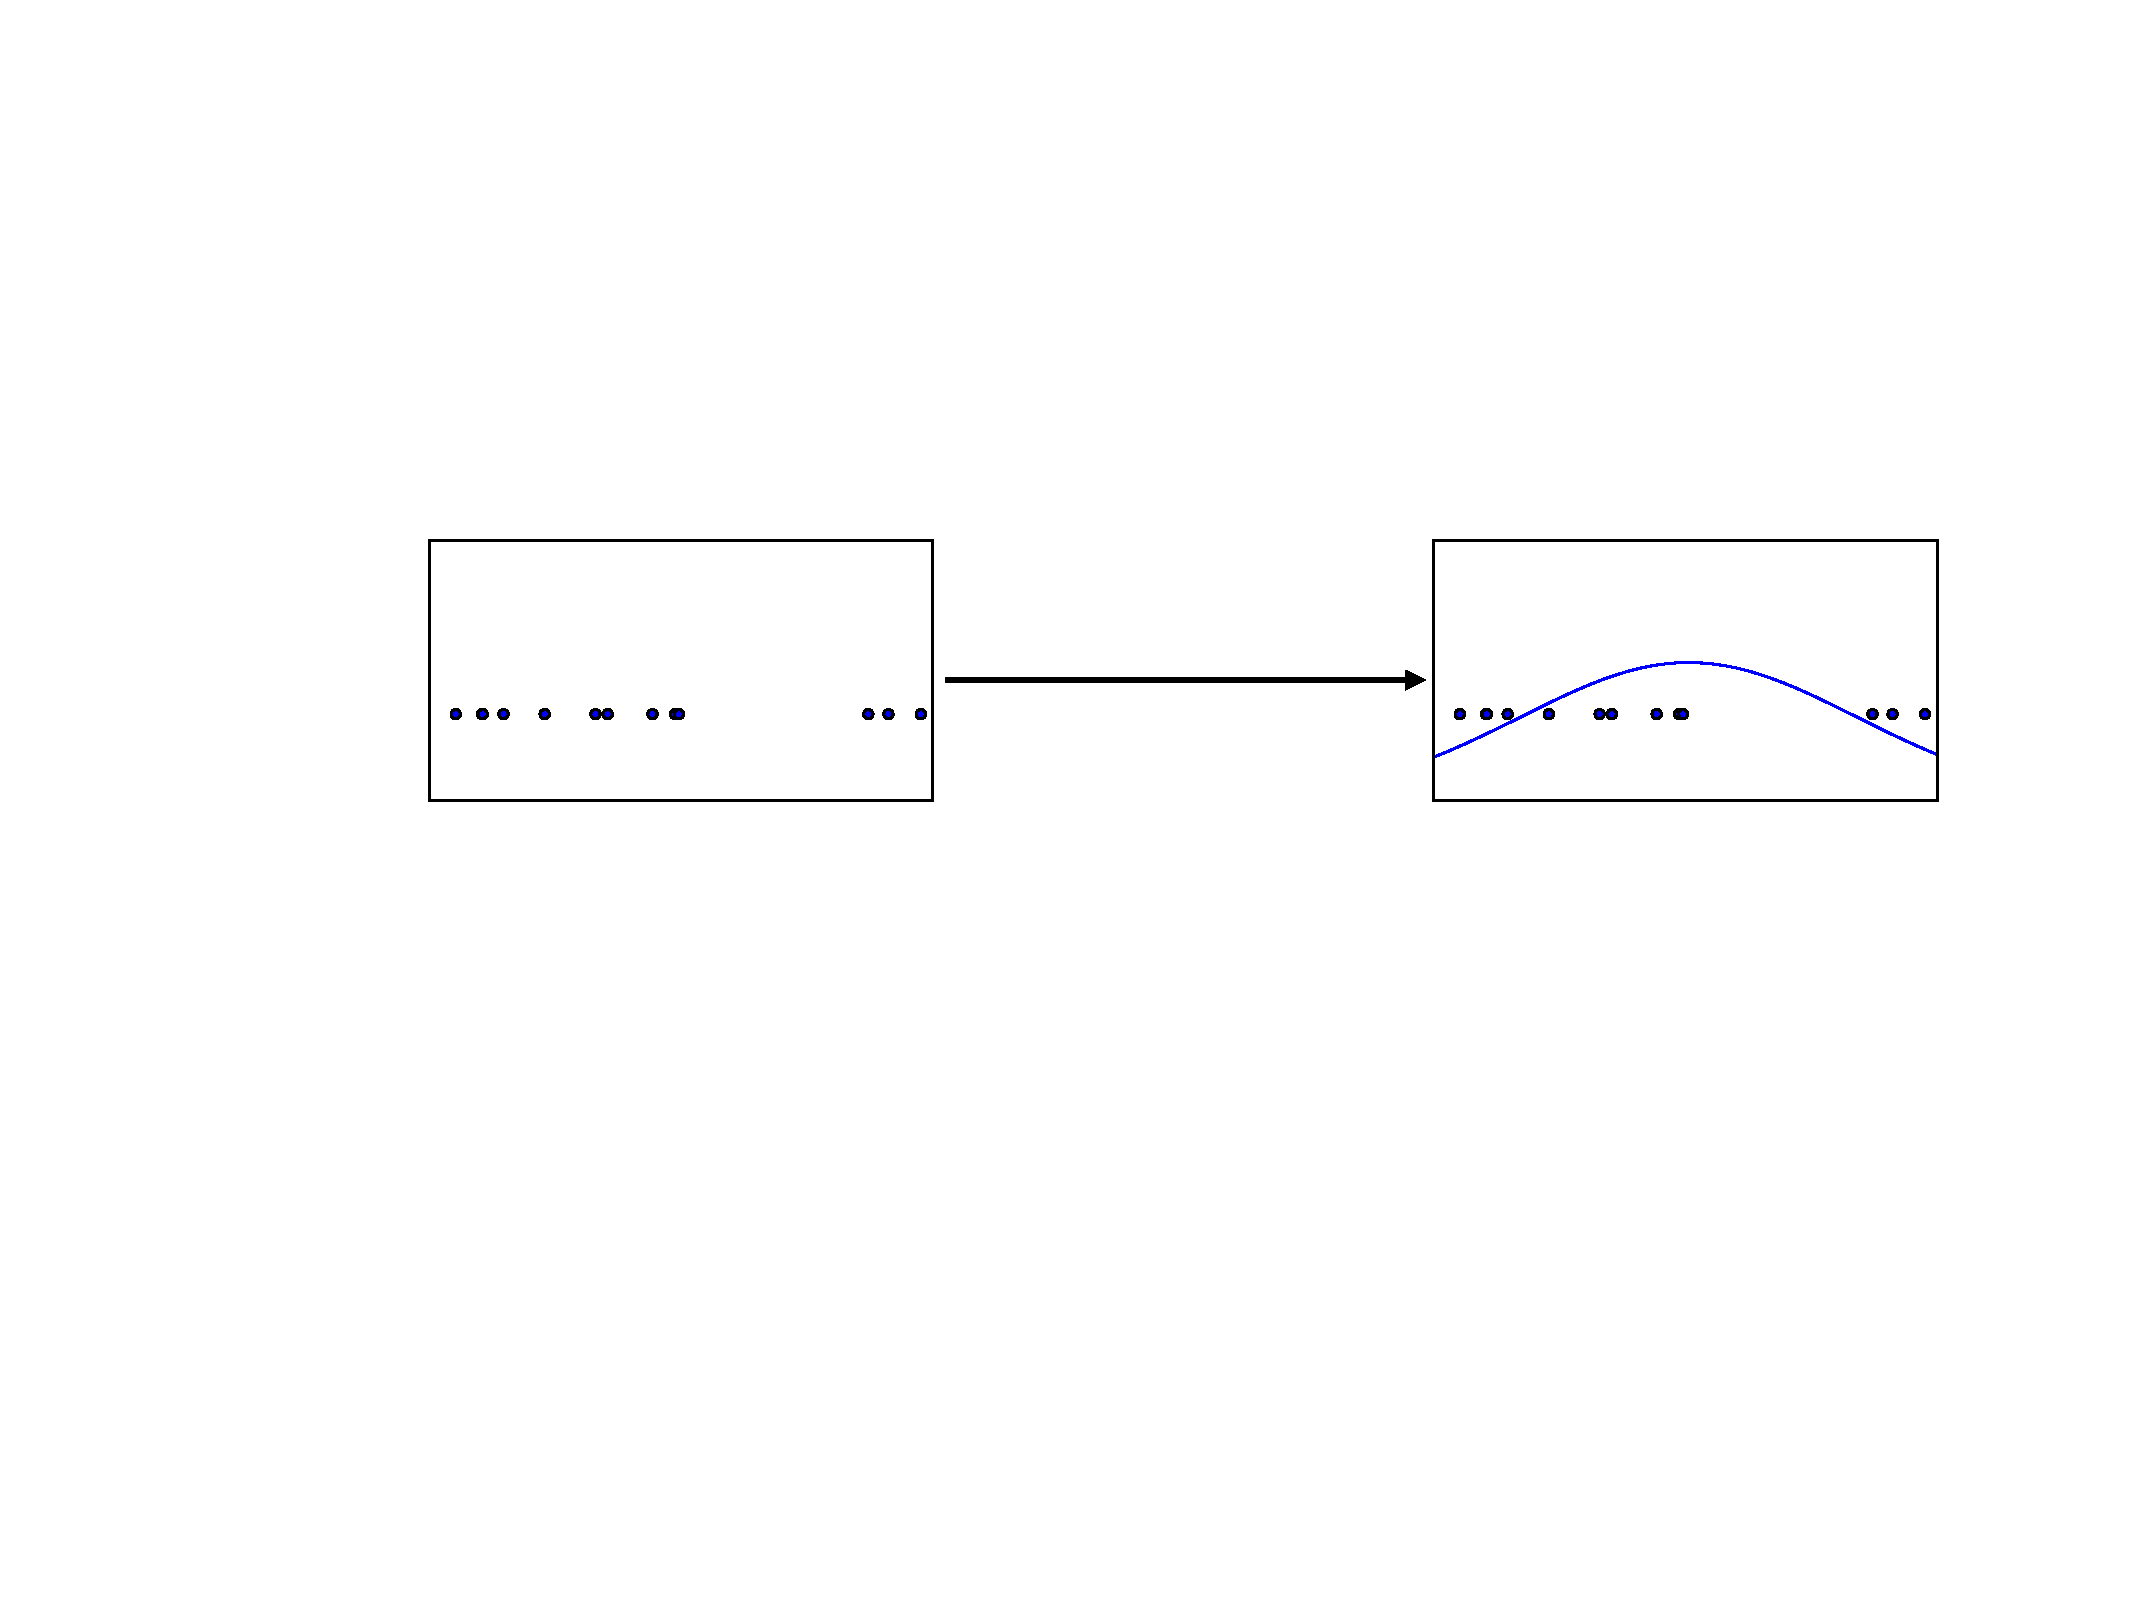
\includegraphics[width=\textwidth]{density.pdf}
\caption{Some generative models perform density estimation.
These models take a training set of examples drawn from an unknown
data-generating distribution $\pdata$ and return an estimate of that
distribution. The estimate $\pmodel$ can be evaluated for a particular
value of $\vx$ to obtain an estimate $\pmodel(\vx)$ of the true
density $\pmodel(\vx)$.
This figure illustrates the process for a collection of samples of
one-dimensional data and a Gaussian model.
}
\label{fig:density}
\end{figure}

\begin{figure}
  \center
  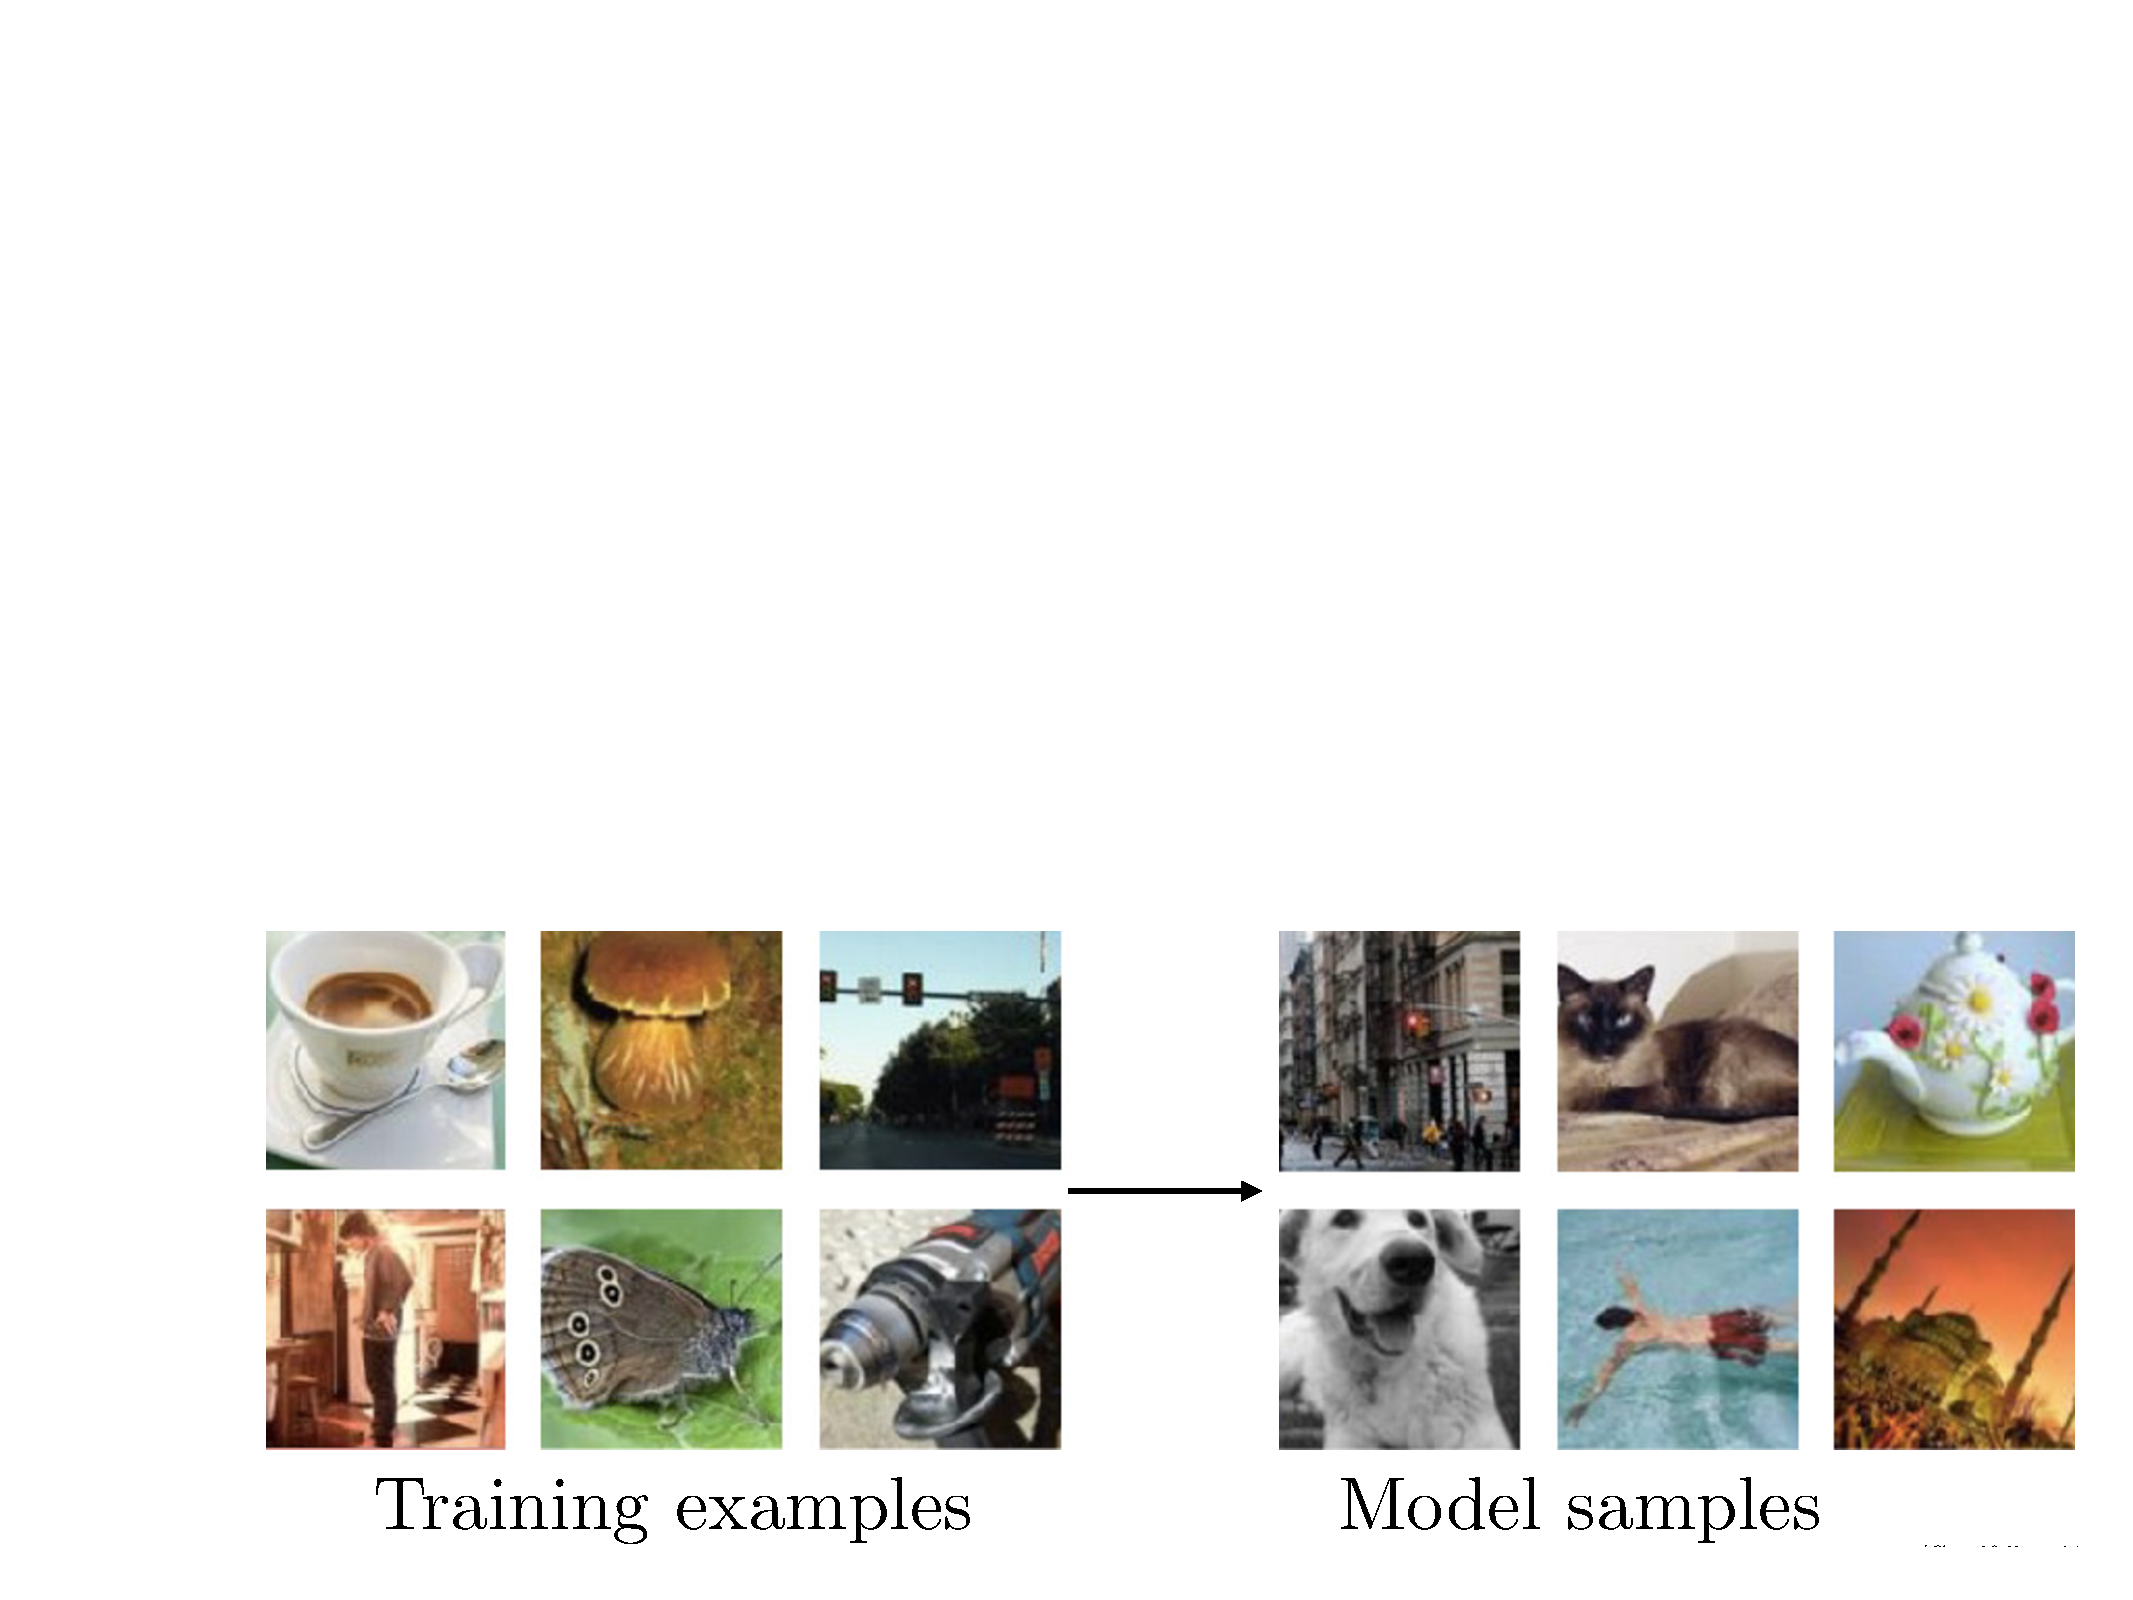
\includegraphics[width=\textwidth]{generative_machine.pdf}
  \caption{Some generative models are able to generate samples
    from the model distribution.
    In this illustration of the process, we show samples from
    the ImageNet \citep{imagenet_cvpr09,Deng2010,ILSVRCarxiv14} 
    dataset.
    An ideal generative model would be able to train on examples
    as shown on the left and then create more examples from the
    same distribution as shown on the right.
    At present, generative models are not yet advanced enough to
    do this correctly for ImageNet, so for demonstration purposes
    this figure uses actual ImageNet data to illustrate what an
    ideal generative model would produce.
  }
  \label{fig:generative_machine}
\end{figure}


\section{Why study generative modeling?}
\label{sec:why}

One might legitimately wonder why generative models are worth studying,
especially generative models that are only capable of generating data
rather than providing an estimate of the density function.
After all, when applied to images, such models seem to merely provide
more images, and the world has no shortage of images.

There are several reasons to study generative models, including:
\begin{itemize}

\item Training and sampling from generative models is an excellent test
of our ability to represent and manipulate high-dimensional probability
distributions.
High-dimensional probability distributions are important objects in a
wide variety of applied math and engineering domains.

\item Generative models can be incorporated into reinforcement learning in several
  ways.
  Reinforcement learning algorithms can be divided into two categories;
  model-based and model-free, with model-based algorithms being those that
  contain a generative model.
  Generative models of time-series data can be used to simulate possible
futures. Such models could be used for planning and for reinforcement learning
in a variety of ways.
A generative model used for planning can learn a conditional distribution over
future states of the world, given the current state of the world and hypothetical
actions an agent might take as input.
The agent can query the model with different potential actions and choose actions
that the model predicts are likely to yield a desired state of the world.
For a recent example of such a model, see \citet{finn2016unsupervised},
and for a recent example of the use of such a model for planning,
see \citet{finn2016deep}. 
Another way that generative models might be used for reinforcement learning is
to enable learning in an imaginary environment, where mistaken actions do not
cause real damage to the agent.
Generative models can also be used to guide exploration by keeping track of
how often different states have been visited or different actions have been
attempted previously.
Generative models, and especially GANs, can also be used for inverse reinforcement
learning.
Some of these connections to reinforcement learning are described further in
TODO.

\item Generative models can be trained with missing data and can provide predictions
  on inputs that are missing data.
  One particularly interesting case of missing data is {\em semi-supervised learning},
  in which the labels for many or even most training examples are missing.
  Modern deep learning algorithms typically require extremely many labeled examples
  to be able to generalize well.
  Semi-supervised learning is one strategy for reducing the number of labels.
  The learning algorithm can improve its generalization by studying a large number
  of unlabeled examples which, which are usually easier to obtain.
  Generative models, and GANs in particular, are able to perform semi-supervised
  learning reasonably well. This is described further in TODO.

\item Generative models, and GANs in particular, enable machine learning to work with
  {\em multi-modal} outputs.
  For many tasks, a single input may correspond to many different correct answers,
  each of which is acceptable.
Some traditional means of training machine learning models, such as minimizing the
mean squared error between a desired output and the model's predicted output, are
not able to train models that can produce multiple different correct answers.
One example of such a scenario is predicting the next frame in a video, as shown
in \figref{fig:lotter}.

\item Finally, many tasks intrinsically require realitic generation of samples from
  some distribution.
\end{itemize}

\begin{figure}
\centering
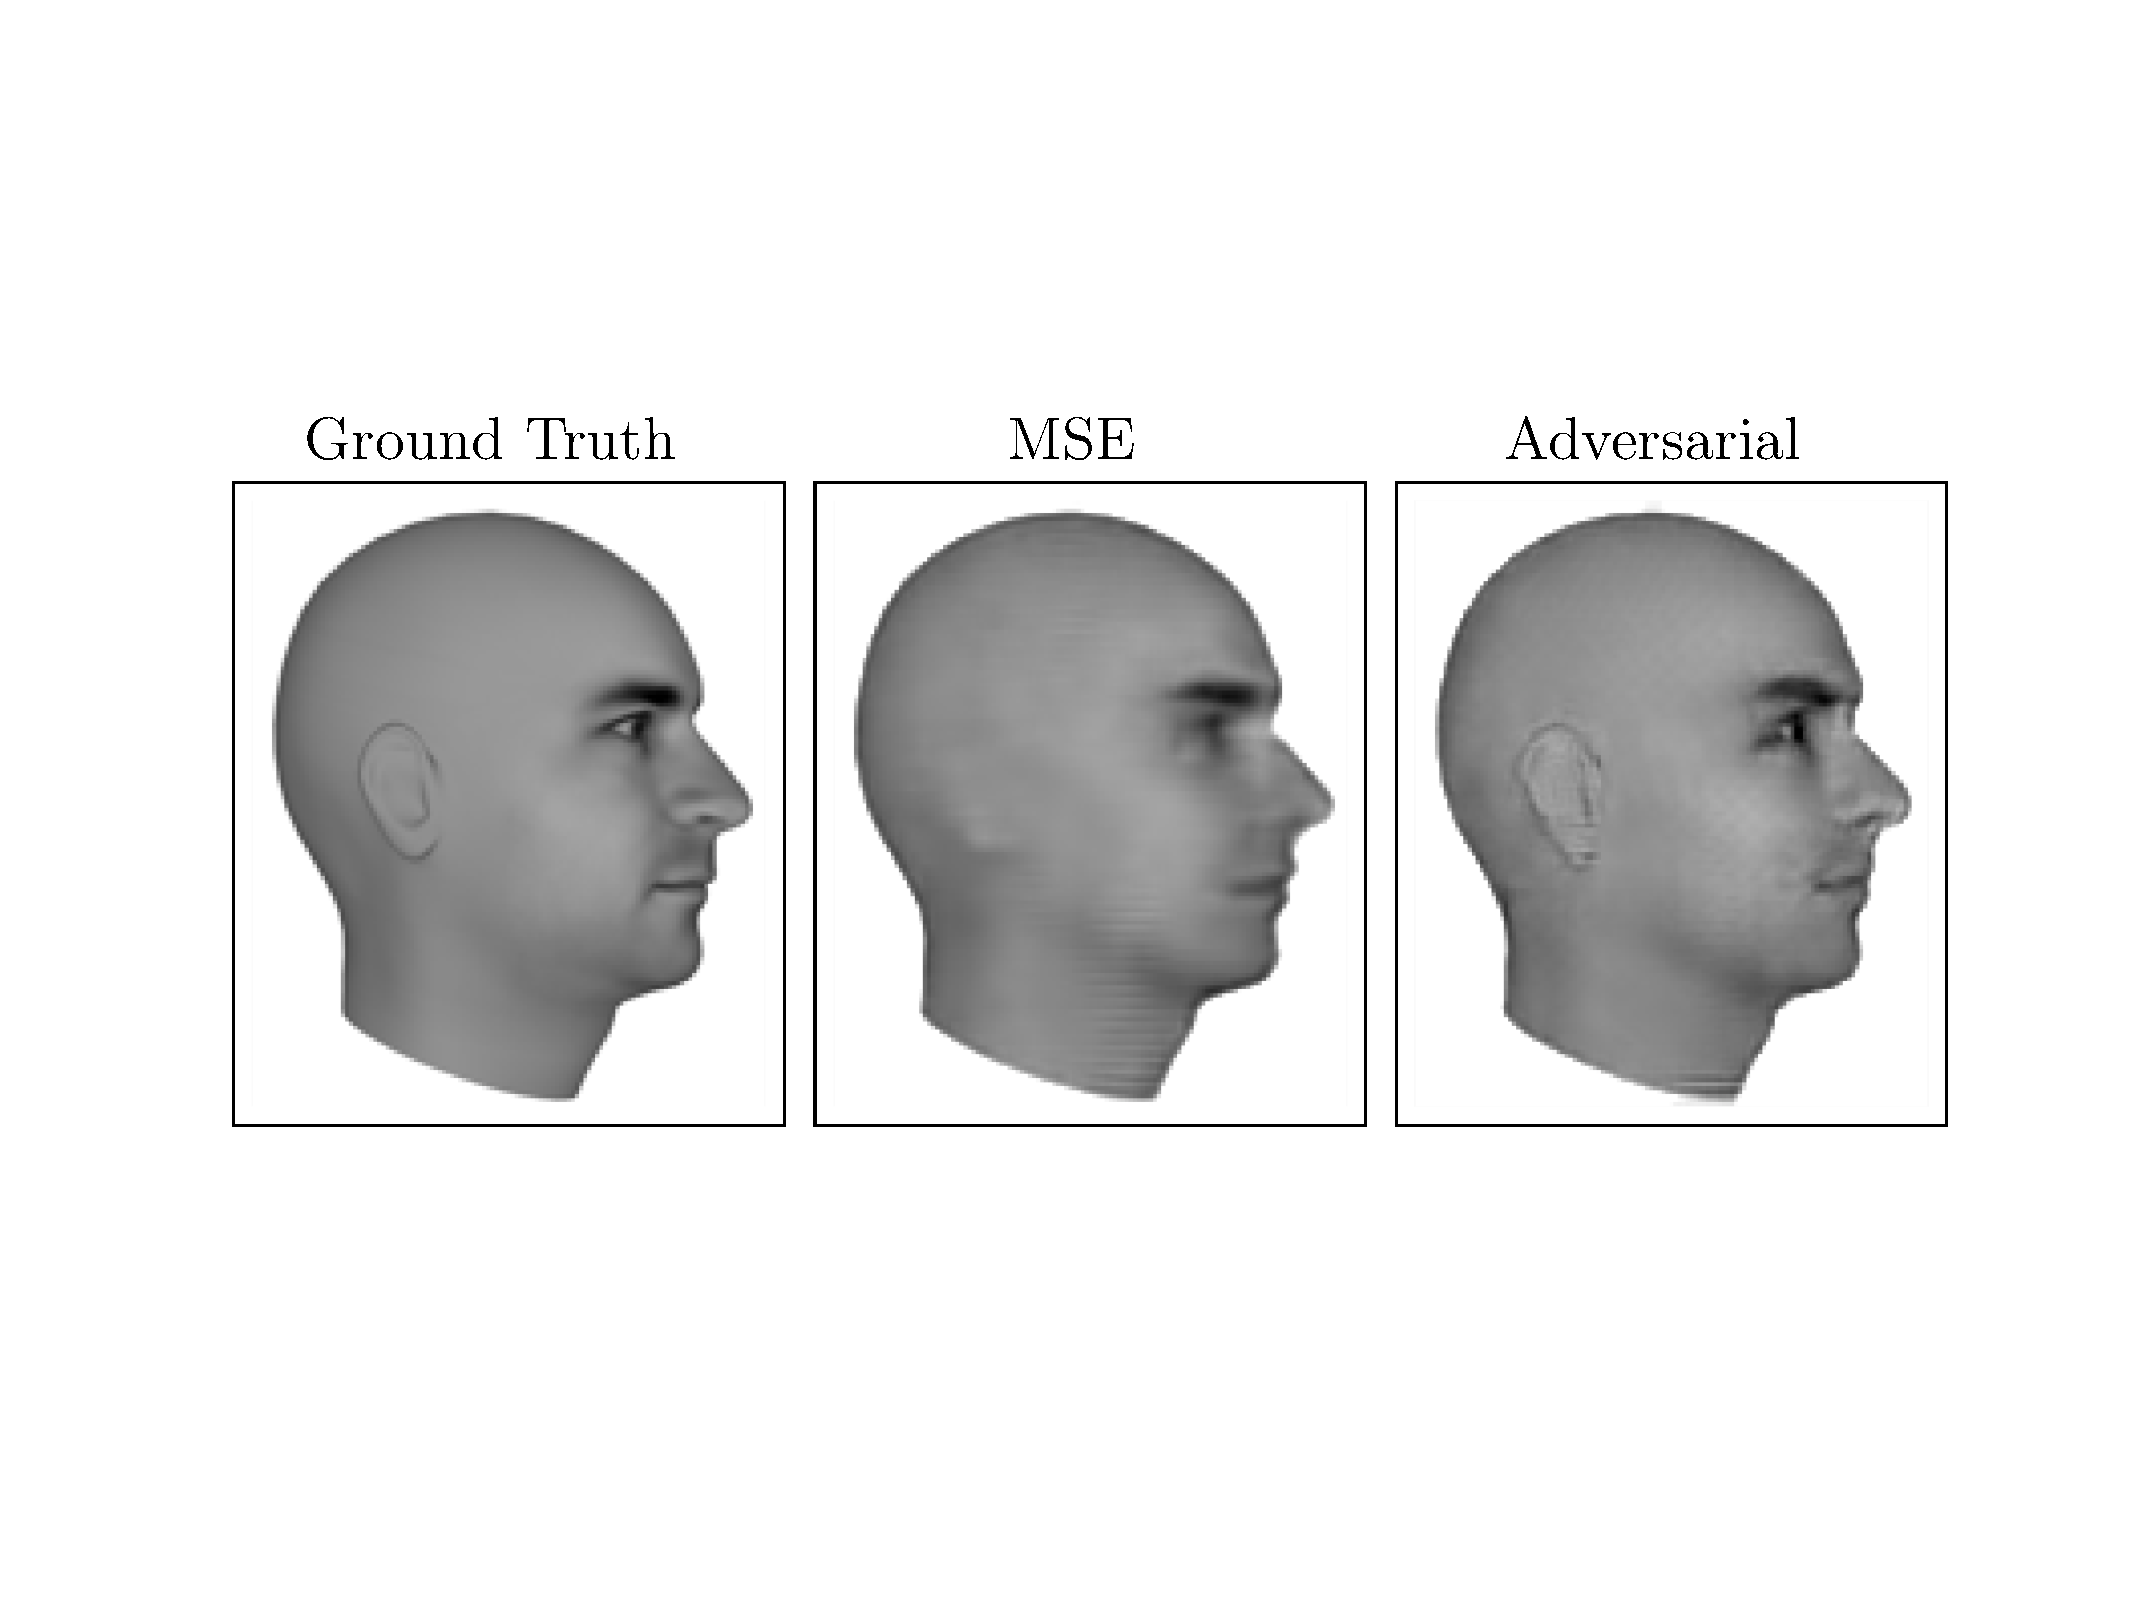
\includegraphics[width=\textwidth]{lotter.pdf}
\caption{
\citet{lotter2015unsupervised} provide an excellent illustration of the importance
of being able to model multi-modal data.
In this example, a model is trained to predict the next frame in a video sequence.
The video depicts a computer rendering of a moving 3D model of a person's head.
The image on the left shows an example of an actual frame of video, which the model
would ideally predict.
The image in the center shows what happens when the model is trained using mean
squared error between the actual next frame and the model's predicted next frame.
The model is forced to choose a single answer for what the next frame will look like.
Because there are many possible futures, corresponding to slightly different positions
of the head, the single answer that the model chooses corresponds to an average over
many slightly different images.
This causes the ears to practically vanish and the eyes to become blurry.
Using an additional GAN loss, the image on the right is able to understand that there
are many possible outputs, each of which is sharp and recognizable as a realistic,
detailed image.
}
  \label{fig:lotter}
\end{figure}

Examples of some of these tasks that intrinsically require the generation of good
samples include:
\begin{itemize}
  \item {\em Single image super-resolution}: In this task, the goal is to take a
    low-resolution image and synthesize a high-resolution equivalent.
    Generative modeling is required because this task requires the model to impute
    more information into the image than was originally there in the input.
    There are many possible high-resolution images corresponding to the low-resolution
    image.
    The model should choose an image that is a sample from the probability distribution
    over possible images.
    Choosing an image that is the average of all possible images would yield a result
    that is too blurry to be pleasing.
    See \figref{fig:superres}.

  \item Tasks where the goal is to create art.
    Two recent projects have both demonstrated that generative models, and in particular,
    GANs, can be used to create interactive programs that assist the user in creating
    realistic images that correspond to rough scenes in the user's imagination.
    See \figref{fig:igan} and \figref{fig:ian}.

\end{itemize}

\begin{figure}
  \centering
  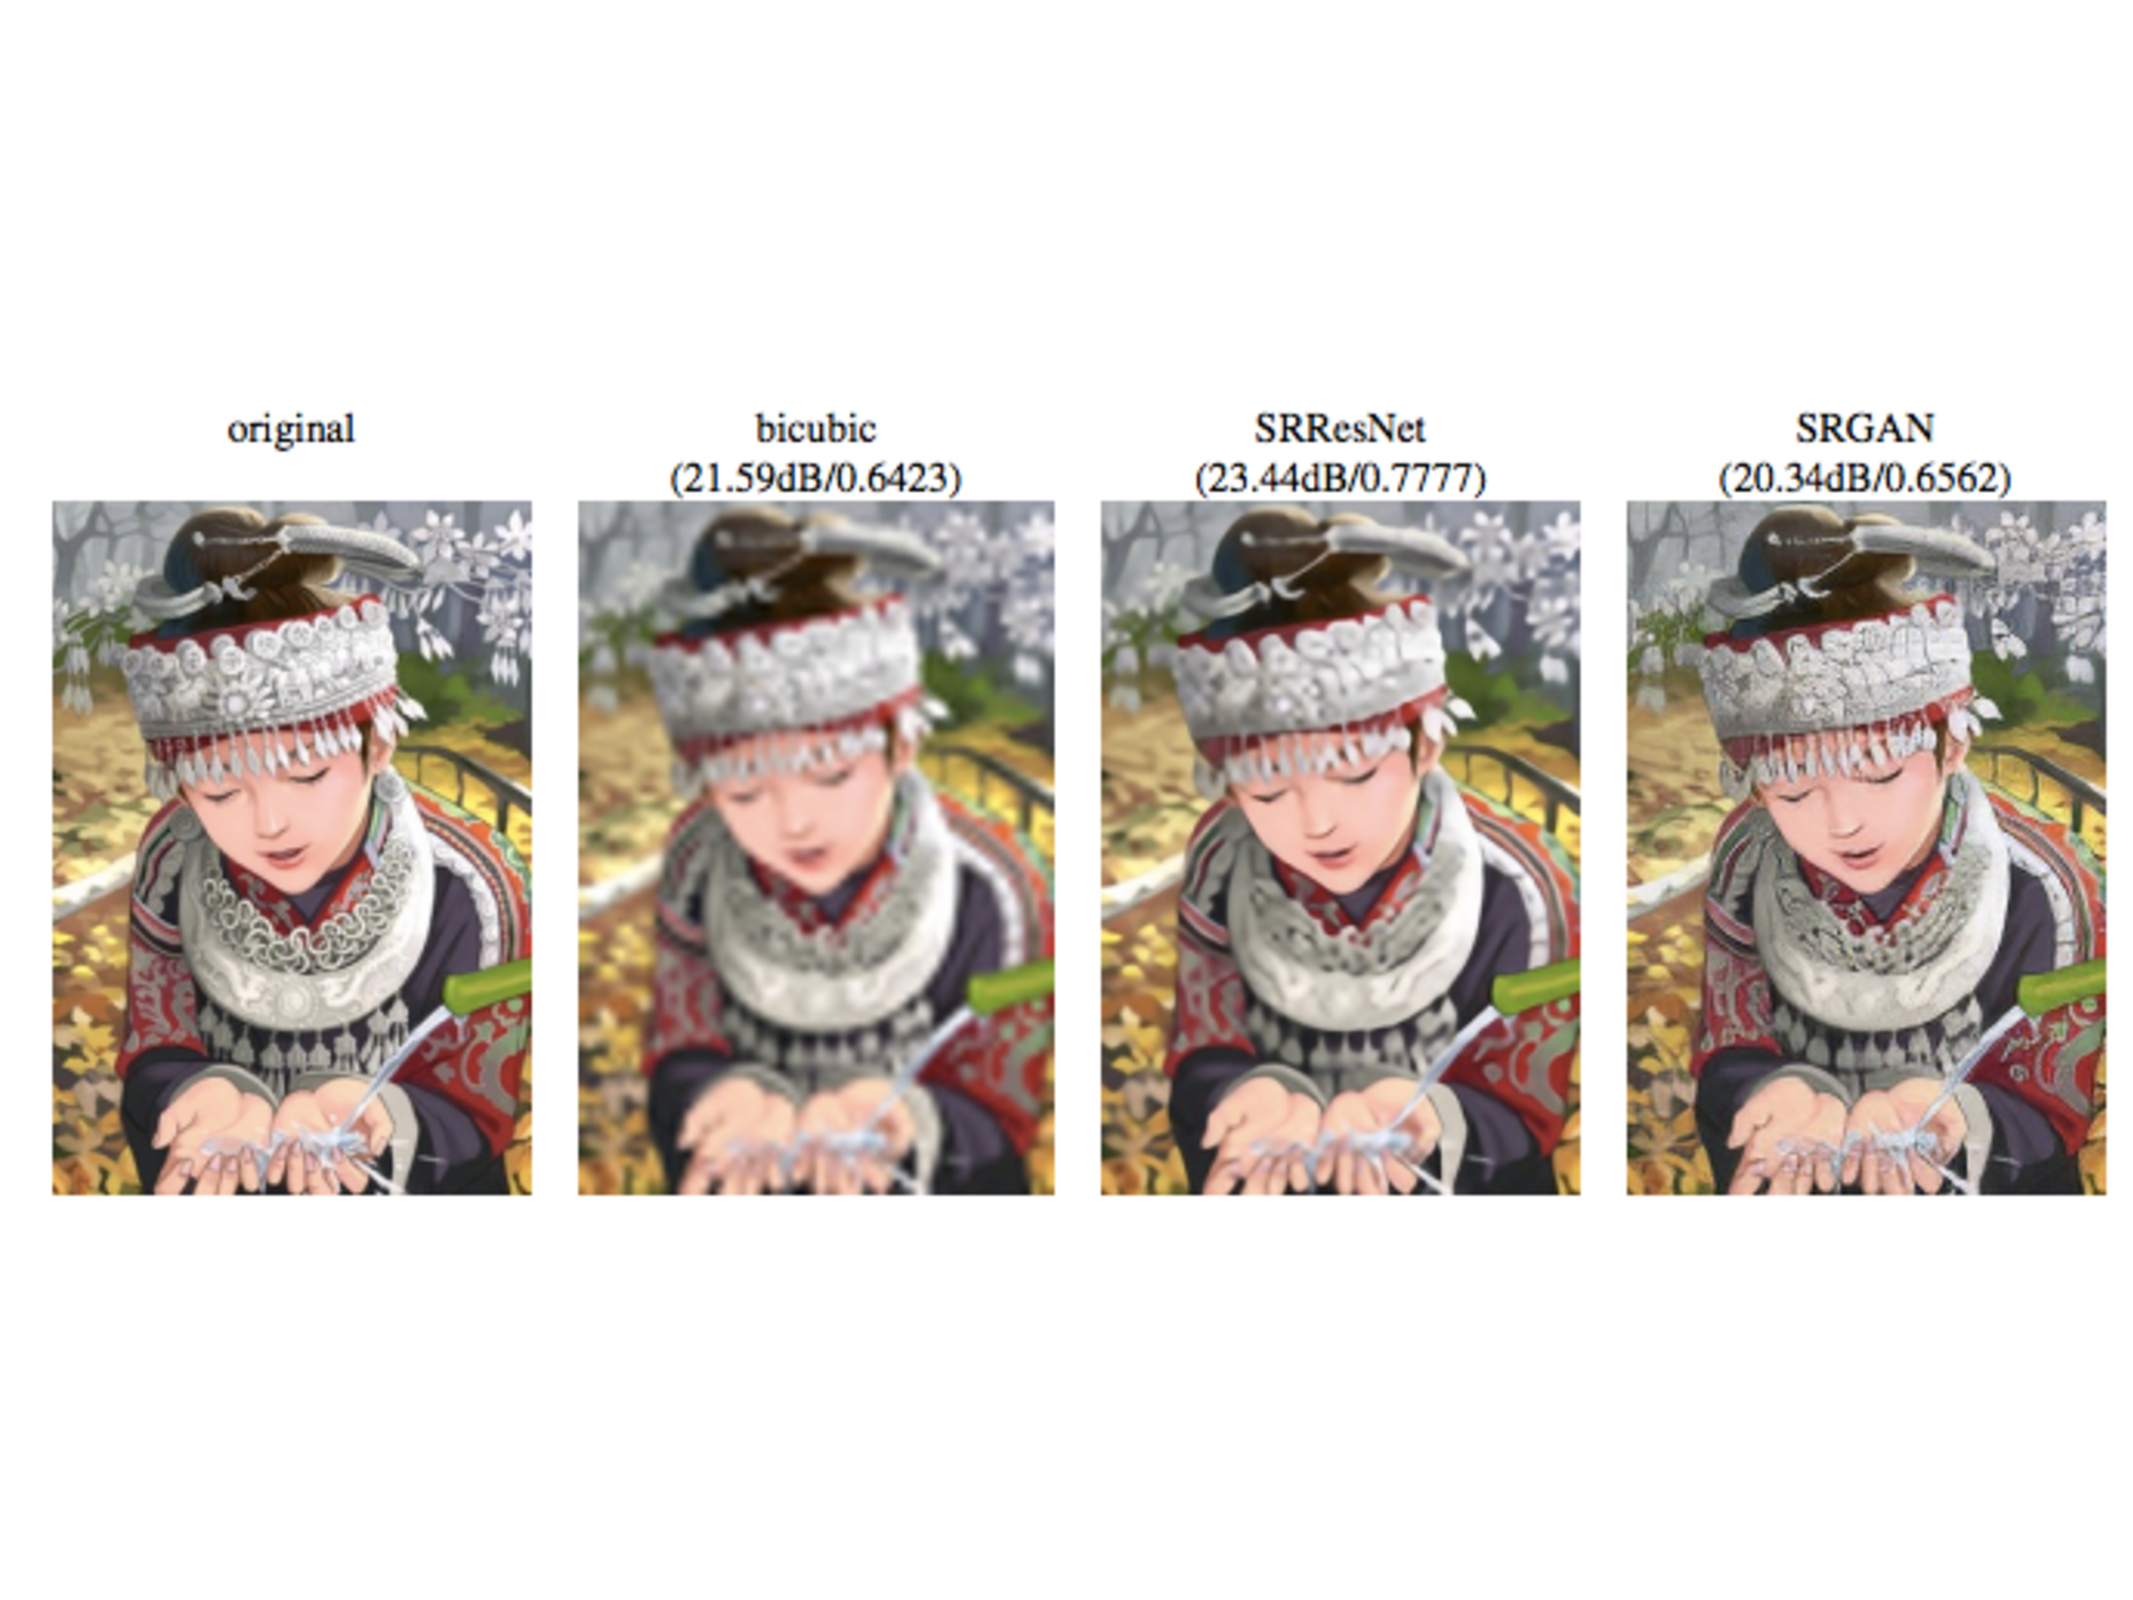
\includegraphics[width=\textwidth]{superres}
  \caption{
\citet{Ledig16} demonstrate excellent single-image superresolution results that show
the benefit of using a generative model trained to generate realistic samples from
 a multimodal distribution.
 The leftmost image is an original high-resolution image.
 It is then downsampled to make a low-resolution image, and different methods
 are used to attempt to recover the high-resolution image.
 The bicubic method is simply an interpolation method that does not use 
 the statistics of the training set at all.
 SRResNet is a neural network trained with mean squared error.
 SRGAN is a GAN-based neural network that improves over SRGAN because it is able
 to understand that there are multiple correct answers, rather than averaging
 over many answers to impose a single best output.
  }
  \label{fig:superres}
\end{figure}

\begin{figure}
  \centering
  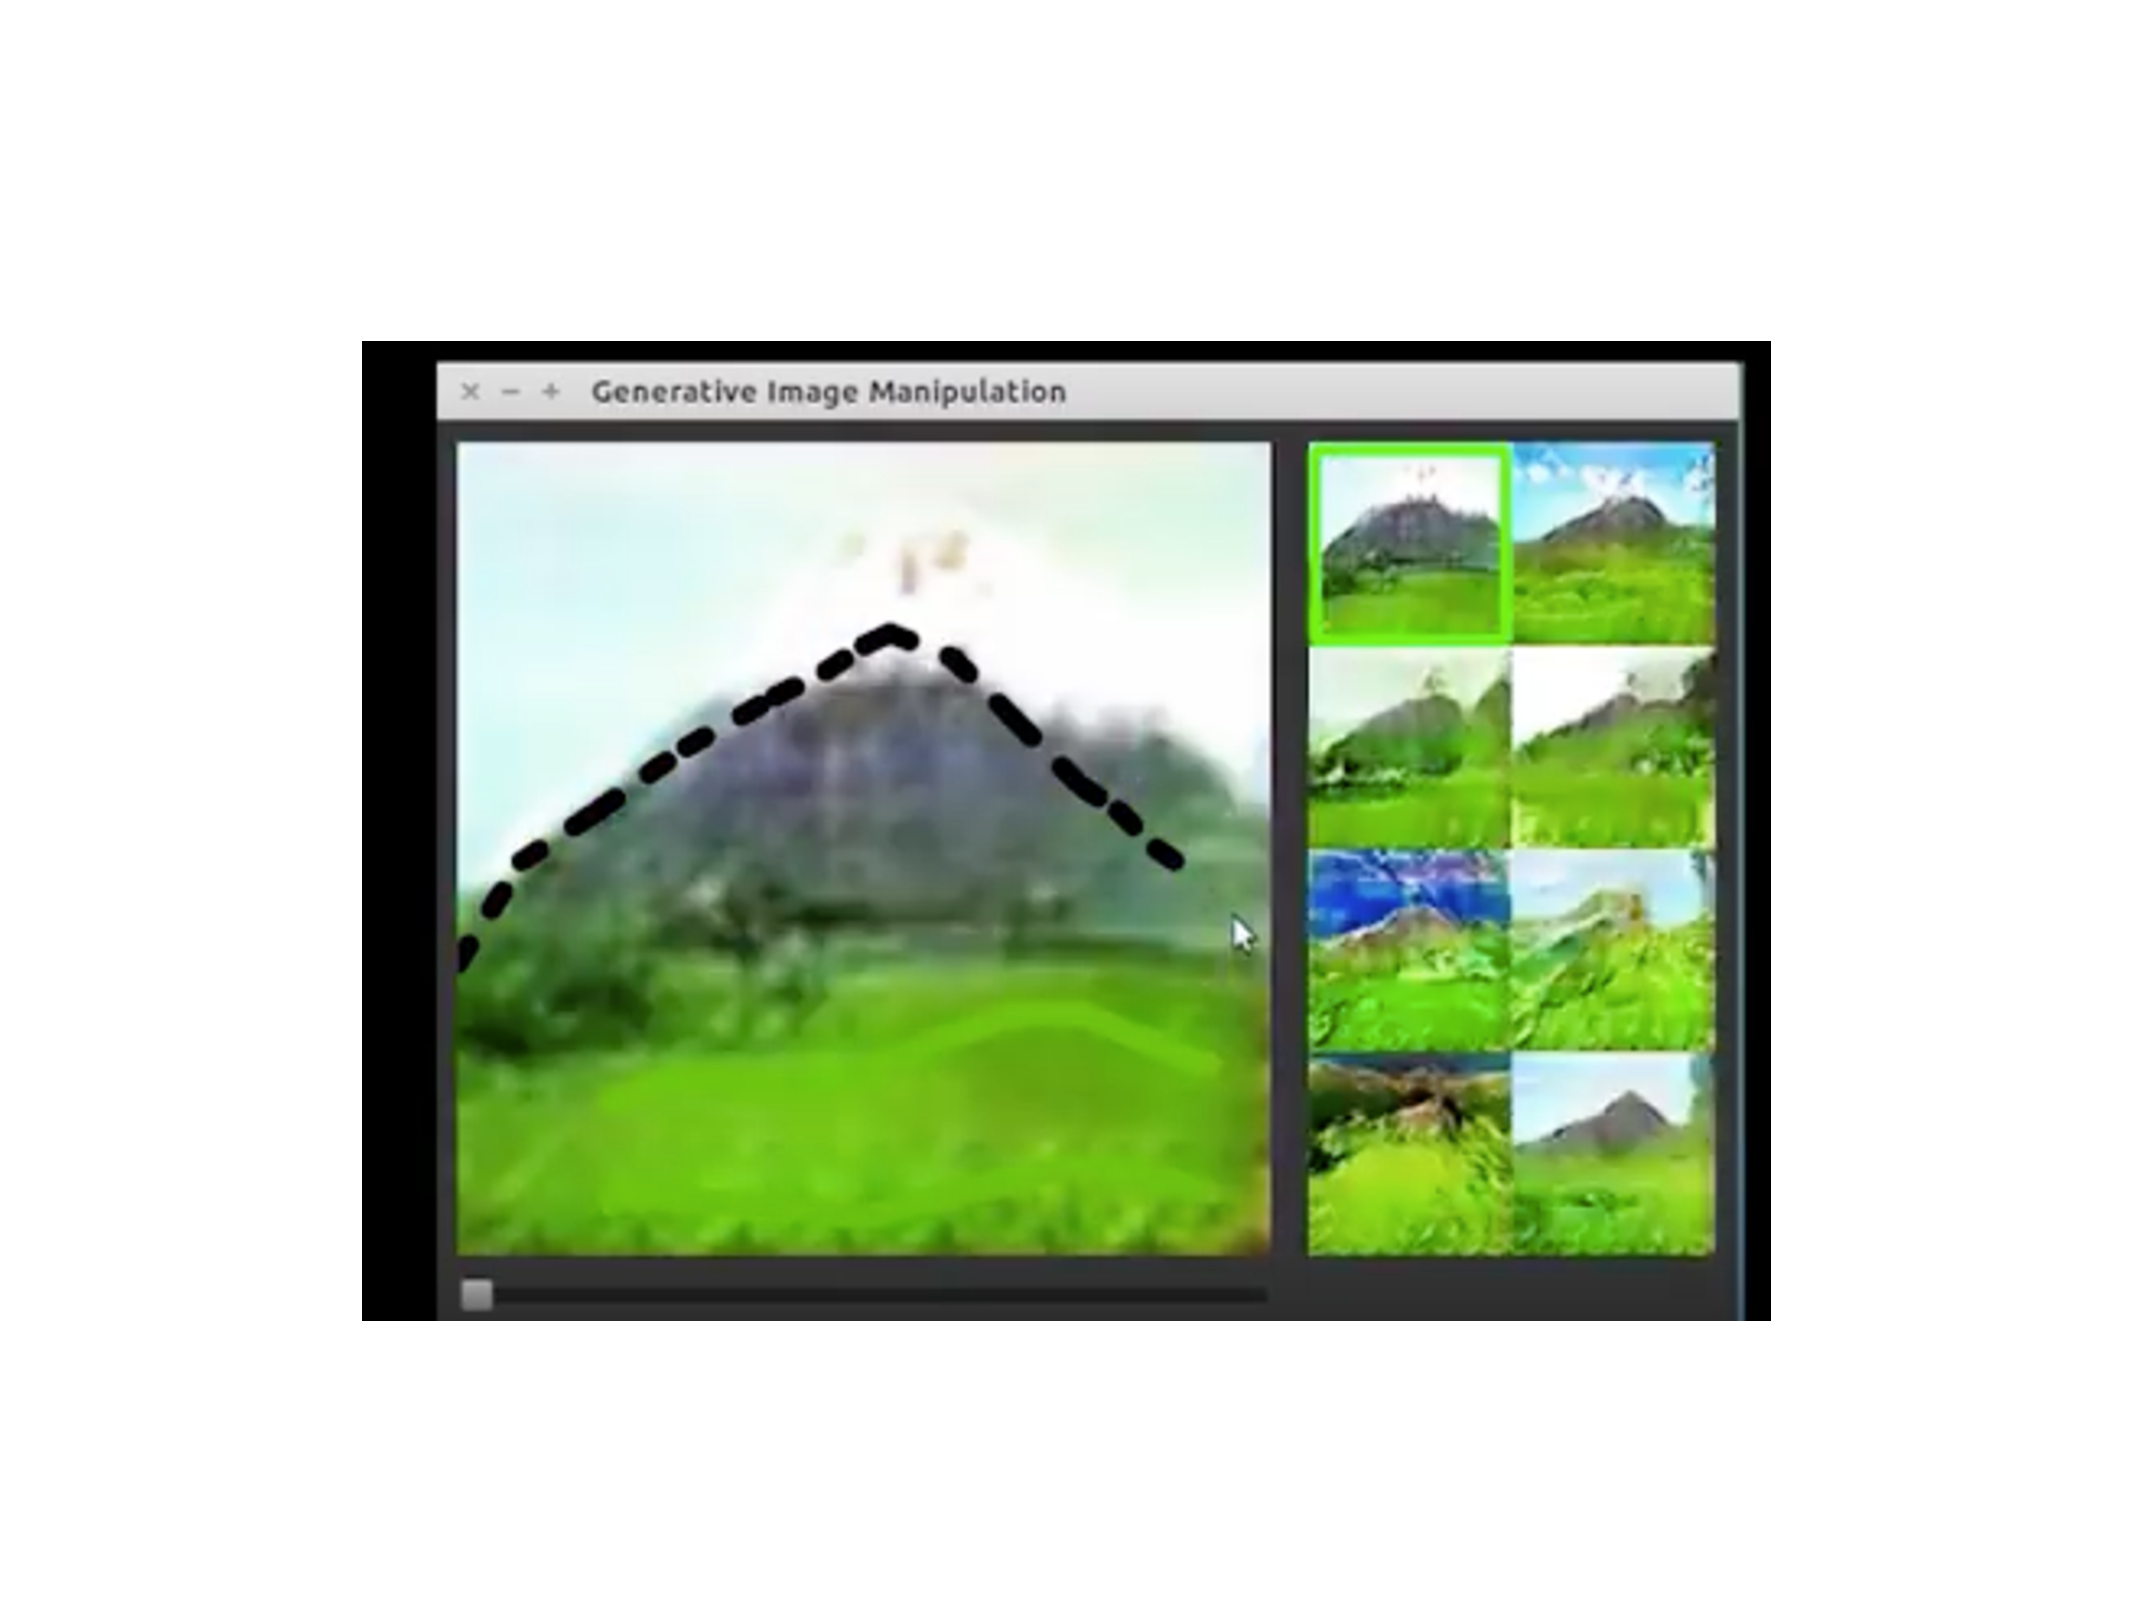
\includegraphics[width=\textwidth]{igan}
  \caption{
TODOcite developed an interactive application called {\em interactive generative adversarial networks}
(iGAN). 
A user can draw a rough sketch of an image, and iGAN uses a GAN to produce the most similar
realistic image.
In this example, a user has scribbled a few green lines that iGAN has converted into a grassy
field, and the user has drawn a black triangle that iGAN has turned into a detailed mountain.
Applications that create art are one of many reasons to study generative models that create
images.
A video demonstration of iGAN is available at the following URL:
\url{https://www.youtube.com/watch?v=9c4z6YsBGQ0}
}
  \label{fig:igan}
\end{figure}


\begin{figure}
  \centering
  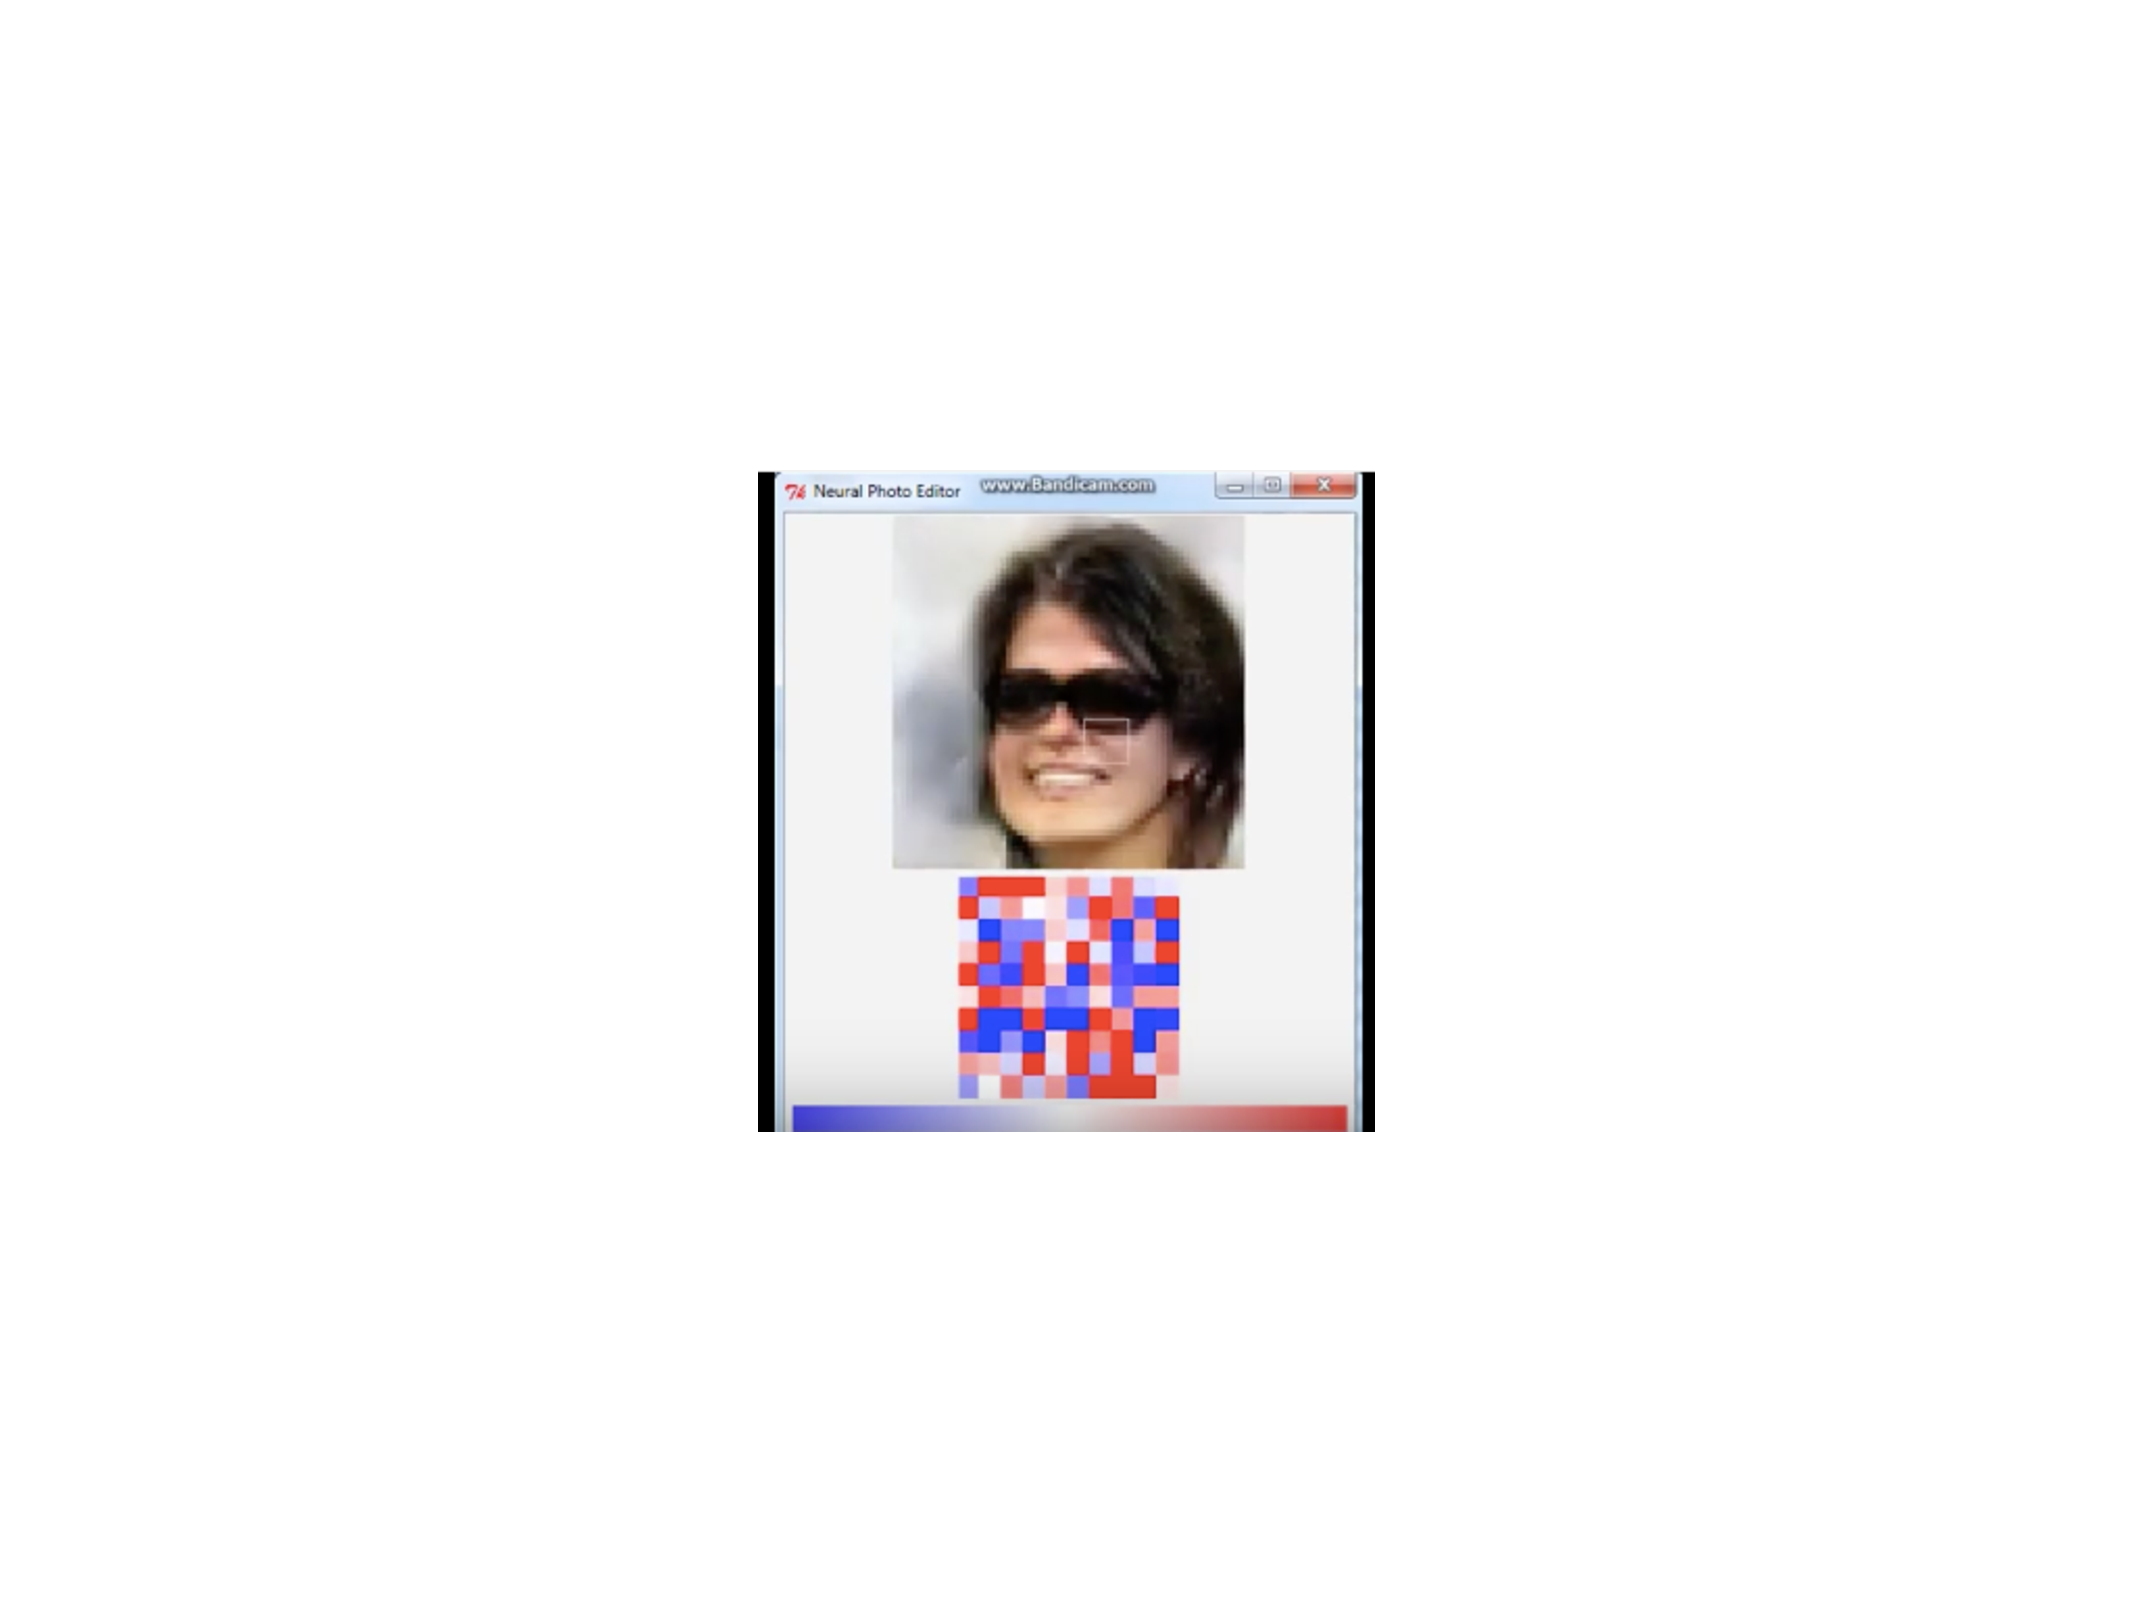
\includegraphics[width=\textwidth]{ian}
  \caption{
    TODOcite developed {\em interactive adversarial networks} (IAN).
    The user paints rough modifications to a photo, such as painting
    with black paint in an area where the user would like to add black
    hair, and IAN turns these rough paint strokes into photorealistic
    imagery matching the user's desires.
    Applications that enable a user to make realistic modifications to
    photo media are one of many reasons to study generative models
    that create images.
    A video demonstration of IAN is available at the following URL:
    \url{https://www.youtube.com/watch?v=FDELBFSeqQs}
  }
  \label{fig:ian}
\end{figure}


\section*{Acknowledgments}
The author would like to thank the NIPS organizers for inviting him to
present this tutorial.
Many thanks also to those who commented on his Twitter and Facebook posts
asking which topics would be of interest to the tutorial audience.


\bibliography{biblio}
\bibliographystyle{natbib}

\end{document}
